
All our experiments were performed on a NUMA machine with 4-sockets each housing a six-core AMD Opteron 8431 processor \cite{opteron}.
Cache related and topology related information about the NUMA hardware can be found at:

\texttt{/sys/devices/system/cpu/cpu*/cache } \\
\\
\texttt{ /sys/devices/system/cpu/cpu*/topology }

The L1, L2 and L3 sizes for the machine were 128, 512 and 6144 KBytes respectively. The following table shows where the
core to socket mapping:

\begin{center}
\begin{tabular}{c|c}
\hline
Socket Id & Core Ids\\
\hline
0 & 0, 4, ..4*i.. 8\\ 
1 & 1, 5, ..4*i+1.. 9 \\
2 & 2, 6, ..4*i+2.. 10\\
3 & 3, 7, ..4*i+3.. 11\\
\hline
\end{tabular}
\end{center}


\subsection{Performance monitoring}
For our measurements, we relied on \texttt{RDTSC} assembly instruction\cite{timeStampCounter} for getting CPU timing information
and \texttt{perf stat} \cite{perfWiki}, for counting the cache misses, page-faults and stalled CPU cycles. We used libnuma,
the NUMA policy library, for control and placement of threads and data on the NUMA nodes. \cite{libNuma} lists many functions
that can be used to modify the default numa policy as required. The command line interface, \texttt{numactl} \cite{numactl} 
provides various command-line arguments like \texttt{cpubind} and \texttt{membind} to bind processes and data to specific nodes.

\subsection{Interconnect Overhead}
Shared code is in essence very similar to read-only data, unless it is self-modifying.
Therefore, all the observations with respect to NUMA overheads for read-only data can be generalized for shared code as well.
In this section, we compute the overhead of fetching the data over the interconnect by comparing the access times for read-only
data for local and remote memory access.

To make our measurements more accurate, we undermine the effect of cpu caches by flushing the cache line associated with the 
variable before every memory access. We do this by using the CLFLUSH\cite{clflush} assembly instruction as follows.


\begin{verbatim}
// ...
const char* roData = "foo";
clflush(roData);
tmp = *roData;
// ...
\end{verbatim}

It should be noted that, if the cpu cache is flushed before the computation, the total ticks elapsed will be the sum of time 
taken to fetch the operand from memory and execute the instruction.
\begin{dmath}
\label{eqn:NoCacheFetch}
T_{CFlush} = T_{MemFetch} + T_{decodeAndExecute}
\end{dmath}

Whereas, if the cache is not flushed, the data is too small and can easily fit in L1 cache, therefore, 
\begin{dmath}
\label{eqn:cacheFetch}
T_{NoCFlush} \approx T_{decodeAndExecute}
\end{dmath}

From \ref{eqn:NoCacheFetch} and \ref{eqn:cacheFetch}, we can compute the value for $T_{MemFetch}$, the
results for which are labeled in the following table (all entries in clock ticks):

\begin{figure}
    \centering
    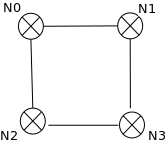
\includegraphics[scale=0.38]{hypercube.png}
    \caption{4-node NUMA topology, N1, N2 and N3 are respectively horizontal, vertical and diagonal neighbors of N0}
    \label{fig:remoteVsLocal}
\end{figure}


\begin{center}
\begin{tabular}{c|c|c|c}
\hline
location & T_{CFlush} & T_{NoCFlush} & T_{MemFetch}\\
\hline
Self & 944 & 330 & 614\\
Horizontal & 1262 & 330 & 932 \\
Vertical & 1258 & 330 & 928\\
Diagonal & 1570 & 330 & 1240\\
\hline
\end{tabular}
\end{center}

From the table above, it can be concluded that adjacent access is 1.5x costly whereas diagonal access is
2x costlier. These observed results agree with the fact that for 4-node NUMA machines, the topology is
hypercube with \textit{C} = 2, as discussed here\cite{Drepper07whatevery}.

\subsection{Library Setup}
We needed to call all the functions in shared library multiple times in different orders. This was difficult
to implement with existing libraries as most functions have different signatures, and therefore, generating
arguments and calling all of them can be a tedious task. To avoid this, we allowed ourselves the flexibility
to generate shared libraries of appropriate sizes using a perl-based code generator or alternatively using
C++ Template Metaprogramming.\cite{templateMeta}

We generated multiple shared libraries, and carried our experiments on them the results of which are presented
in the next section. All the functions in the library were indexed in a \textit{functionTable}, from where they
could be called in various different ways.
